\textbf{A.\quad Perguntas do questionário fechado aos alunos:}
\begin{enumerate}
    \item Você é um aluno(a) da Engenharia de Software?
    Alternativas: Sim ou não
    
    \item Qual o seu sexo biológico?
    Alternativas: Feminino ou Masculino
    
    \item Qual a sua faixa etária?
    Alternativas: Abaixo de 18 anos; 18 a 24 anos; 25 a 35 anos; 35 a 45 anos; Acima de 45 anos
    
    \item Em que período da graduação você se encontra? 
    Alternativas: 1º a 8º período
    
    \item Há quanto tempo você trabalha na área?
    Alternativas: Não trabalho na área ainda; Até 2 anos na área; 2 a 4 anos na área; 4 a 6 anos na área; Mais de 6 anos na área

    \item Numa escala de 1 a 5, em que 1 representa "Insatisfeito" e 5 representa "Muito satisfeito", como você classifica sua satisfação com o aprendizado proporcionado pela atividade proposta?
    Alternativas: de 1 a 5
    
    \item Numa escala de 1 a 5, em que 1 representa "Aprendi pouco" e 5 representa "Aprendi muito", como você classifica o aprendizado que a atividade proposta foi capaz de oferecer?
    Alternativas: de 1 a 5
    
    \item Numa escala de 1 a 5, em que 1 representa "Pouco interesse" e 5 representa "Muito interesse", como você classifica o seu interesse na atividade proposta?
    Alternativas: de 1 a 5
    
    \item Numa escala de 1 a 5, em que 1 representa "Baixo" e 5 representa "Alto", como você classifica seu nível de cumprimento da atividade proposta?
    Alternativas: de 1 a 5
    
    \item Numa escala de 1 a 5, em que 1 representa "Muito fácil" e 5 representa "Muito difícil", como você classifica o nível de dificuldade enfrentado na realização da atividade proposta?
    Alternativas: de 1 a 5
    
    \item Numa escala de 1 a 5, em que 1 representa "Tempo insuficiente" e 5 representa "Tempo mais que suficiente", como você classifica o tempo disponibilizado para a realização da atividade proposta?
    Alternativas: de 1 a 5
    
    \item Numa escala de 1 a 5, em que 1 representa "Pouco próximo" e 5 representa "Muito próximo", como você classifica a proximidade da atividade proposta em relação às práticas e demandas profissionais do mercado?
    Alternativas: de 1 a 5
    
    \item Numa escala de 1 a 5, em que 1 representa "Não ajudou" e 5 representa "Ajudou muito", o quanto você julga que a atividade proposta ajudou na sua compreensão de problemas reais envolvendo o tema da atividade?
    Alternativas: de 1 a 5
    
    \item Numa escala de 1 a 5, em que 1 representa "Não agregou" e 5 representa "Agregou muito", o quanto você julga que a atividade proposta agregou em sua vida profissional?
    Alternativas: de 1 a 5
\end{enumerate}
\textbf{B.\quad Perguntas do questionário fechado aos professores:}
\begin{enumerate}
    \item Numa escala de 1 a 5, na qual 1 representa ``Não estão engajados" e 5 representa ``Estão muito engajados", como você classifica o engajamento que os alunos apresentaram em relação à atividade prática?
    Alternativas: de 1 a 5
    
    \item Numa escala de 1 a 5, na qual 1 representa ``Baixa" e 5 representa ``Alta",  como você classifica a complexidade envolvida na realização da atividade proposta?
    Alternativas: de 1 a 5
    
    \item Numa escala de 1 a 5, na qual 1 representa ``Insatisfatório" e 5 representa ``Muito satisfatório", como você classifica o desempenho que os alunos apresentaram na atividade proposta?
    Alternativas: de 1 a 5
    
    \item Numa escala de 1 a 5, na qual 1 representa ``Pouca dificuldade" e 5 representa ``Muita dificuldade", qual é a sua percepção do nível de dificuldade que os alunos tiveram para executar a atividade prática?
    Alternativas: de 1 a 5
    
    \item Numa escala de 1 a 5, na qual 1 representa ``Pouca proximidade" e 5 representa ``Muita proximidade", qual é a sua percepção do nível de proximidade existente entre a atividade proposta e as práticas e demandas profissionais do mercado?
    Alternativas: de 1 a 5
\end{enumerate}
\textbf{C.\quad Perguntas do questionário aberto aos alunos:}
\begin{enumerate}
    \item Discuta sua percepção geral sobre a atividade prática proposta (dificuldades, aprendizados, pontos positivos e/ou negativos). Busque se expressar sobre tópicos abordados e não abordados pelo questionário fechado.
    
    \item Você tem considerações que possam contribuir para melhorar a atividade, na sua opinião? Caso tenha, por favor, tente se basear na resposta dada à pergunta anterior para responder a esta pergunta.
\end{enumerate}
\textbf{D.\quad Problemas de programação (prática 2):}
\begin{enumerate}
\item Escreva um programa ou método que receba como entrada um vetor de inteiros e imprima como saída o número que representa a moda (ou seja, o número com maior ocorrência no vetor).

\item Escreva um programa ou método que receba como entrada um número inteiro e  imprima como saída o valor de seu fatorial.

\item Escreva um programa ou método que receba como entrada um número inteiro em base decimal e imprima como saída seu valor em binário.

\item Escreva um programa ou método que receba como entrada um número inteiro N e imprima como saída os N primeiros termos da sequência de Fibonacci.
\end{enumerate}
\textbf{E.\quad Links:}

Questionário fechado dos alunos:
http://bit.ly/Fechado-Alunos

Questionário fechado do professor:
http://bit.ly/Fechado-Professores

Questionário aberto dos alunos:
http://bit.ly/Aberto-Alunos

Problemas de programação:
https://bit.ly/tcc-pratica2

\textbf{F.\quad \textit{Script}:}
\begin{figure}
    \centering
    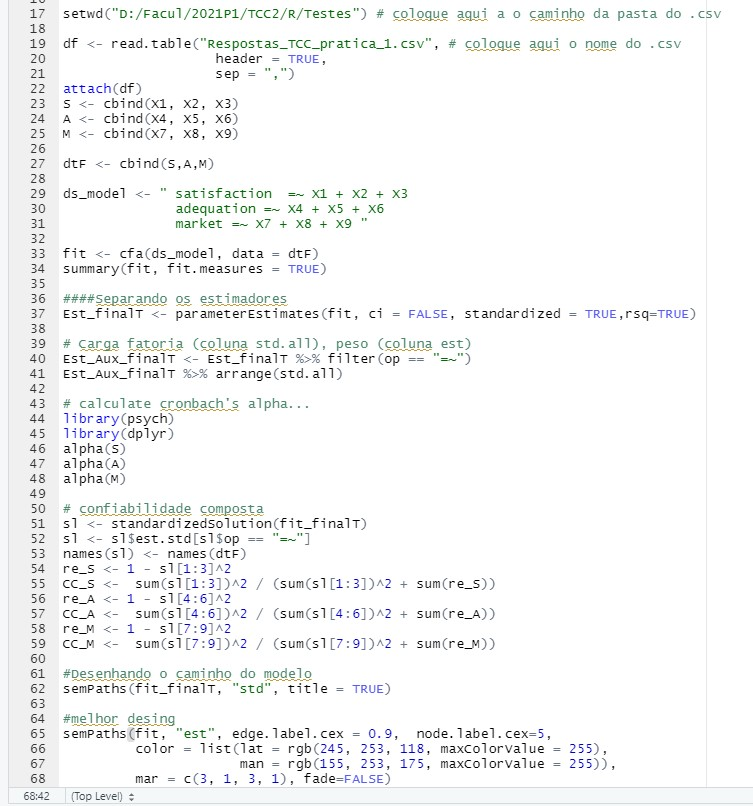
\includegraphics[width=12cm,height=12cm]{Imagens/script.jpg}
    \caption{\textit{script} elaborado em R}
    \label{fig:Processo}
\end{figure}

\ \